\documentclass{jdrp}

\bibliography{dos-au-muur/references} 

\newcommand*{\crg}{{\aurebesh\Large \$}} % Symbol for Galactic Credits

\hypersetup{
	pdftitle={SWR - Dos au Muur},
	pdfsubject={Scénario, Dos au Muur},
	pdfauthor={Marthym},
	pdfkeywords={starwars,savage,worlds,jdr,scenario},
	pdfcopiright={This work is licensed under the Creative Commons Attribution-ShareAlike 4.0 International License.}
}

\begin{document}

	\begin{titlepage}

	\begin{center}
		\hspace*{\vfill}
		\noindent\Huge\jedifont{Star Wars Redemption}\\ 
		\noindent\fontsize{50}{70}\jedifont{\$}
		\noindent\fontsize{50}{70}\jedifont{\#}\\
		\noindent\fontsize{50}{60}\jedifont{Dos au Muur}
		\hspace*{\vfill}
	\end{center}

	\hspace*{\vfill}

	\noindent\makebox[\textwidth]{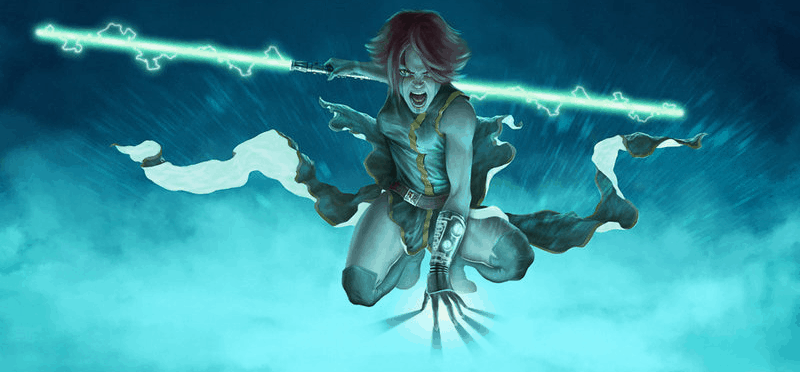
\includegraphics[width=\paperwidth]{_img/cover-bg.png}}

	\end{titlepage}

\section{contexte de campagne}
La campagne se déroule dans les premières années de l'avènement de l'Empire, au MJ de voir s'il veut préciser.

L'objectif de la campagne est de retrouver un très ancien artéfact, le \textbf{Talisman de Muur}. Un artéfact créé par Karness Muur, un Sith se servant de la Force pour prolonger sa vie. L'artéfact contient l'âme de Muur, celui qui le porte est possédé par Karness et peut contrôller les Rakghoules.

Mais nous verrons plus en détails au cours de la quête.

	\section{Sauvetage du Pelican}

Voici un scénario d'introduction pour la campagne \textbf{Dos au Muur}. Cette campagne est écrite initialement pour \citetitle{jdrp-starwars} mais un scénar reste un scénar et il est jouable dans n'importe quel univers de Star Wars.

Il est adaptable aussi bien avec des joueurs orienté Alliance Rebelle que Empire. Dans les deux cas, l'objectif sera le même mais les dessains changeront.

La campagne est faite pour des joueurs débutant, partant du rang Novice.

\vspace{2\baselineskip}
\begin{flushright}
	\emph{Pelican (IA-1701)}
\end{flushright}

\vspace{-4\baselineskip}

\hspace{-0.4\columnsep}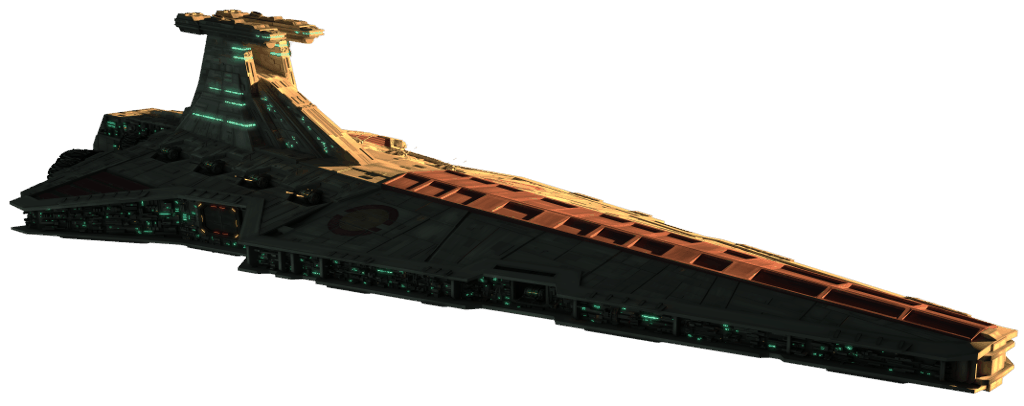
\includegraphics[width=\textwidth]{_img/dos-au-muur/venator.png}
\vspace{-7\baselineskip}

\subsection{La rencontre}
Nos héros ne se connaisent pas encore. Ils ont répondu à un contract proposé par \emph{Industrial Automaton} pour une mission de récupération.

Ils ont rendez-vous sur l'avant poste commercial de l'anneau de Kafrene au Starlord Café. \'A leur arrivé, ils sont conviés dans une arrière salle ou les attend Vyna Anen un Sluissi, le représentant de IA. En plus du groupe de nos héros, deux autres personnes ont répondu au contract, un Abyssin et un Rodien.

\begin{quote}
	Messieurs bonjour, je représente Indrustrial Automaton.
	Comme vous avez peu le voir sur le contract auquel vous avez répondu, nous cherchons a rassembler une équipe pour récupérer l'un de nos prototype de droïde Type R perdu sur Croiseur dont nous n'avons plus de nouvelle.
	Le \textbf{Pelican IA-1701} n'a plus donné signe de vie depuis 10h et 33mn maintenant. Il avait a son bord le seul prototype de notre dernier Type R. Il est vital pour nous de récupérer ce prototype intact.

	Si vous acceptez la mission, une navette droïde vous conduira directement à la dernière position connu du Pelican. Cette mission doit resté confidentielle, nous ne tenons pas à ce que le public sache qu'Industrial Automaton perde ses vaisseau !
	En cas de succés la somme convenue sera virée directement sur vos comptes respectif. Dans le cas contraire vous serez mort ou en passe de l'être.

	Il y a t'il des questions ?

	\ldots

	Bien, la navette décollera de l'astroport, quai N°5 dans une heure, elle n'attendra personne.
\end{quote}

Voilà qui donne le ton et la direction du scénario. Les héros disposent donc d'une heure, s'ils le souhaitent pour faire quelques amplettes puis direction la navette.

\subsection{Pelican Bay}
\'A la sortie d'hyperespace, les héros trouvent croiseur de classe Venator en bon état mais à la dérive. La navette tente une procédure d'appomtage mais le système de guidage ne semble pas fonctionner, le droïde aux commande de la navette ne cesse de répéter 

\begin{flushright}
		Erreur trop bas tros bas !\\
		Erreur trop bas tros bas !\\
		Erreur trop bas tros bas !\\
		Erreur trop bas tros bas !\\
		\ldots
\end{flushright}

\vspace{5\baselineskip}
Et la navette s'échoue lamentablement dans le hangard. Comme de par hasard, et pour bien appuyer sur le gravité de la situation, l'Abyssin et le Rodien sont mort pendant le crash et le droïde pilote est dans un sale état. Il ne pourra donner aucune information.

Une fois à bord du Pelican, une alarme est en cours et une voie pré-enregistré se fait entendre à intervale régulier :

\begin{quote}
	Alerte trajectoire, le vaisseau se dirige actuellement vers une étoile, point de non retour dans 2h53mn ! 
	Voyez modifier la trajactoire du vaisseau !\\ 
	\ldots
\end{quote}

\'A l'intérieur du vaisseau c'est la désolation, des cadavres partout, du sang sur les murs, des traces de griffures sur les murs. L'éclairage est partiellement en panne les neons scintilles, des débrits entravent la marche des héros. Leur champ de vision est réduit à cause des conditions à bord. Malgrés tout ça, les systèmes de survit et la gravité artificielle fonctionne.\\

Le bruit du crash de la navette a attiré la population locale, a savoir les Rakghouls~\ref{sec:rakghoul} (p. \pageref{sec:rakghoul}). Lancer 1d4 pour savoir combien se pointent. Si vous n'avez que 2 ou trois héros sous la main, ajustez avec 1d4-1.

\noindent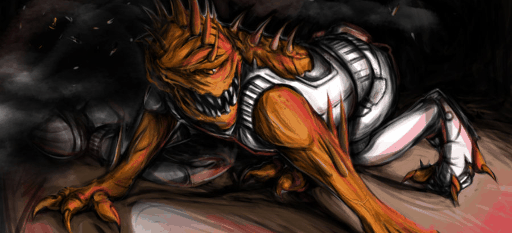
\includegraphics[width=\linewidth]{_img/dos-au-muur/rakghoul.png}

Le but des héros devrait maintenant être double, trouver le fameux prototype mais aussi trouver un moyen de sauver leur peau. 

\subsection{Exploration}
\emph{Numéroté les pièces de votre vaisseau et lancez un dé pour savoir dans qu'elle pièce se trouve le droïde.}\\

Une fois la première vague de Rakghouls balayé, nos héros se retrouvent dans le hangard, la porte de se dernier est ouverte.

Un jet de Recherche (-2 pour l'obscurité) réussi permet de trouver un kit de survie avec un Medipack, une lampe torche et des ratio de survie.

Pas loin de la porte du hangard se trouve un terminal dont l'écran clignote en rouge au rythme de l'alarme. Les héros peuvent tenter des jet de Piratage pour les actions suivantes :
\begin{rebelist}
	\item Stopper l'alarme. 
	\item Obtenir un plan du vaisseau. En cas de succés, le plan s'affiche mais le terminal rend l'âme au bout de quelques secondes et le plan s'efface. En cas de relance le plan reste affiché et le terminal est utilisable.
	\item  Obtenir l'inventaire des navettes présentent dans le hangard du vaisseau. Un succès leur apprend qu'il y en a une dans le hangard du niveau inférieur. Une Relance leur apprend que la navette est dans le hangard 4-2.
\end{rebelist}
Dans tout les cas, un échec critique fait disjoncter le terminal définitivement.

Les héros avancent donc dans les couloirs du Pelican à la recherche du droïde et d'un moyen de dévier le vaisseau. Faites faire un jet de Discrétion de temps à autre. En cas d'échec, 2 Rakghouls se pointent (plus si vous voyez que vos héros s'en tire trop facilement).

Au fur et mesure que les aventuriers avancent, utilisez les tuiles pour découvrir la carte du vaisseau.

\subsubsection{Le Droïde}
Quand les héros arrivent dans la salle où se trouve le droïde, ce dernier les menace avec un arc électrique, rien de bien méchant mais les héros doivent le rassurer et Négocier (jet de Persuasion) avec le droïde ou le Pirater (jet de Piratage opposé à l'Intellect). Dans les deux cas, avec un succés, le droïde les aide, leur montre le journal de bord. Avec un relance, le droïde devient un accolyte du héros qui a fait l'action. En cas d'échec le droïde refuse de les aider il se désactive. En cas d'échec critique, le droïde s'en prend à eux.

Si le droïde se désactive, un héros peut tenter de lui retirer la mémoire pour récupérer les infos avec un jet de Réparation. 

\subsubsection{Les Quartiers}
Il s'agit des quartiers de l'équipage. Pas grand chose à y trouver, des vètements, des effets personnels. On y trouve des terminaux qui peuvent être Piraté pour le plan du vaisseau ou pour d'auters information. Avec un succès, ils se connectent et ont accès au contenu du PC. La carte s'ils la cherche, sinon rien de fou, des photos, des vidéos et des films X.

\subsubsection{Les Laboratoires}
La porte du premier labo que les héros visitent est verrouillé. un jet de Piratage la déverrouille. Si le droïde est avec eux et les aide, il peut ouvrir toutes les portes. Les aventuriers trouvent dans ce labo le corps corps du rakghoul et un terminal. Un Piratage (malus -2, c'est un terminal sécurisé) leur donne les informations sur l'autopsie (cf. Le journal de bord~\ref{sec:pelican-jdb} p. \pageref{sec:pelican-jdb}), pas plus sur les circonstances.

Dans les autres labo, un jet de recherche donne un Medipac supplémentaire.

\subsubsection{L'Armurerie}
Dans cette pièce se trouve des cellules énergétiques pour les armes et des armes mais enfermées dans des casiers. Un coup de blaster ouvre les casiers. On trouve alors 5x Blaster Semi-Automatique (2d8 (3)) et 1x Lance Grenade (2d10 (1)), 5x Grenade (3d6).


\subsubsection{Le Pont}
La pièce est verrouillée et ne peut être ouverte avec un Piratage. Seul le droïde peut l'ouvrir. Si le droïde disparait ou s'éteind, la salle s'ouvre. Les héros en entrant dans la pièce trouvent le corp sdécomposé du commandant. En recherchant dans les poches du commandant, ils trouvent un document marqué "Protocole d'Urgence" expliquand la marche à suivre en cas de problème (cf. Le journal de bord~\ref{sec:pelican-jdb} p. \pageref{sec:pelican-jdb}). Le papier contient aussi les les codes d'accès au terminal.

Les héros peuvent donc accéder au journal de bord~\ref{sec:pelican-jdb} p. \pageref{sec:pelican-jdb}) avec toutes les infos. Si cela n'est déjà connu, ils savent qu'un vaisseau en état les attends dans le hangard 4-2 et il est possible d'en ouvrir la porte depuis ce terminal. S'ils sont malin, il est possible de voir ce qui les attends dans le hangard via des caméra de surveillance. Il peuvent aussi déclencher l'autodestruction.

\begin{paperbox}{Objectifs}
Les joueurs doivent d'une manière ou d'une autre apprendre l'histoire des rakghoul et du Talisman. Donc soit par le droïde, soit par le pont. Une fois qu'une des deux étapes est faite, l'autre n'est pas obligatoire. Donc peu importe qu'il déglinguent le droïde.
\end{paperbox}

\subsection{Le Hangard 4-2}

\noindent
\includegraphics[width=\linewidth]{_img/dos-au-muur/rakghoul-amblyope.png}

Situé au pont inférieur, deuxième hangard. C'est l'étape final et le boss de fin du scénario.

Le droïde ou un passage au poste de commande déverrouille la porte du handard. \'A l'intérieur c'est une autre histoire, une créature de 2m de haut manifestement un rakghoul aux stéroïdes, un rakghoul Amblyope~\ref{sec:rakghoul-amblyope} p. \pageref{sec:rakghoul-amblyope}).

Selon vos héros et leur état, accompagnez le joker avec quelques rakghouls en extra. Les héros avec Sens de Force ressentent une forte présence du coté obscur autour de la créature.\\

Une fois le combat terminé, il ne leur reste plus qu'a prendre le vaisseau (Cargo léger YZ-775). Ouf, les clefs sont sur le contact. L'armement du vaisseau est endommagé et ne fonctionne pas mais le reste est intact.

\subsection{To be continue\ldots}
Une fois en vol, vos héros reçoivent une communication d'origine inconnue, le visage d'une femme apparait

\begin{quote}
	Tinon \emph{(prononcer Taïnon)} c'est toi ? Que se passe t'il ou va tu ?
\end{quote}

Rideau, suite au prochain épisode\ldots

%http://www.starwars-holonet.com/encyclopedie/technologie-talisman-muur.html

\clearpage
\section{Pelican (iA-1701)}

Quelques information sur le Pelican. C'est un croiseur de classe Venator. 1 137 m de long, 7400 hommes d'équipage, capable d'hyperpropulsion.

Le Pelican appartien à Industrial Automaton qui s'en sert comme vaisseau scientifique ultra-sécurisé. Ils y hébergent des projets top secret et au limite de la loi.

\subsection{Journal de bord}
\label{sec:pelican-jdb}
En relation étroite avec l'Empire, Industrial Automation envoie le Pelican à la recherche d'un ancien artéfact Sith, le Talisman de Muur. Le Pelican à fini par trouver une trace du Talisman sur Taris mais le Talisman n'y est plus, par contre en fouillant les bas fonds de la planète, l'équipe de chercheur trouve un temple Sith. Mais ce dernier est infesté de Rakghouls. L'unité de sécurité qui accompagne les chercheurs parvient à se débarrasser des quelques créatures mais plusieurs hommes sont blessés pendant le combat. Dans les ruines du temple le Talisman n'est plus là mais des indices tendent à penser qu'il a été transporté il y a très longtemps vers \emph{Jebble} (Planète glacière dans la bordure extérieure). Les scientifiques décident de ramener l'un des corps de Rakghoul à bord du Pelican pour l'étudier.

En chemin vers Jebble les scientifiques étudient le corps du Rakghoul et apprennent qu'il s'agit d'une maladie artificielle créé il y a des millénaire par Karness Muur. La maladie se transmet par griffure ou morçure. Cette maladie est étroitement liée à la Force et il semble que les personnes sensibles à la force ne puissent être contaminées. Cependant le Rakghoul étudié a l'air d'être contaminé par une forme très basique du virus, certainement une exposition prolongé à l'artéfact.

Après une semaine de voyage, les problèmes ont commencés. Les soldats blaissés lors de la rixe contre les Rakghouls sur Taris commencent à se transformer en Rakghouls à leur tour et s'en prennent au membre de l'équipage. C'est une boucherie sans nom. Voyant ça, le commandant du Pelican enregistre le journal de bord sur un droïde Type R et tente de bloquer le cap du vaisseau sur l'étoile la plus proche mais la propulsion est endommagé et bien que la cap du vaisseau soit bloqué, ce dernier se contante de dériver.

\subsection{Industrial Automaton}
N'ayant plus de nouvelle du Pelican depuis son départ de Taris, IA part à sa recherche. Ils le retrouve et envoient une équipe mais là encore, plus aucune nouvelles. C'est alors qu'IA décide d'envoyer des mercenaires. Si le commandant à respecté le protocole, il suffira que les mercenaires ramène le droïde\ldots

\subsection{Plan du vaisseau}
\noindent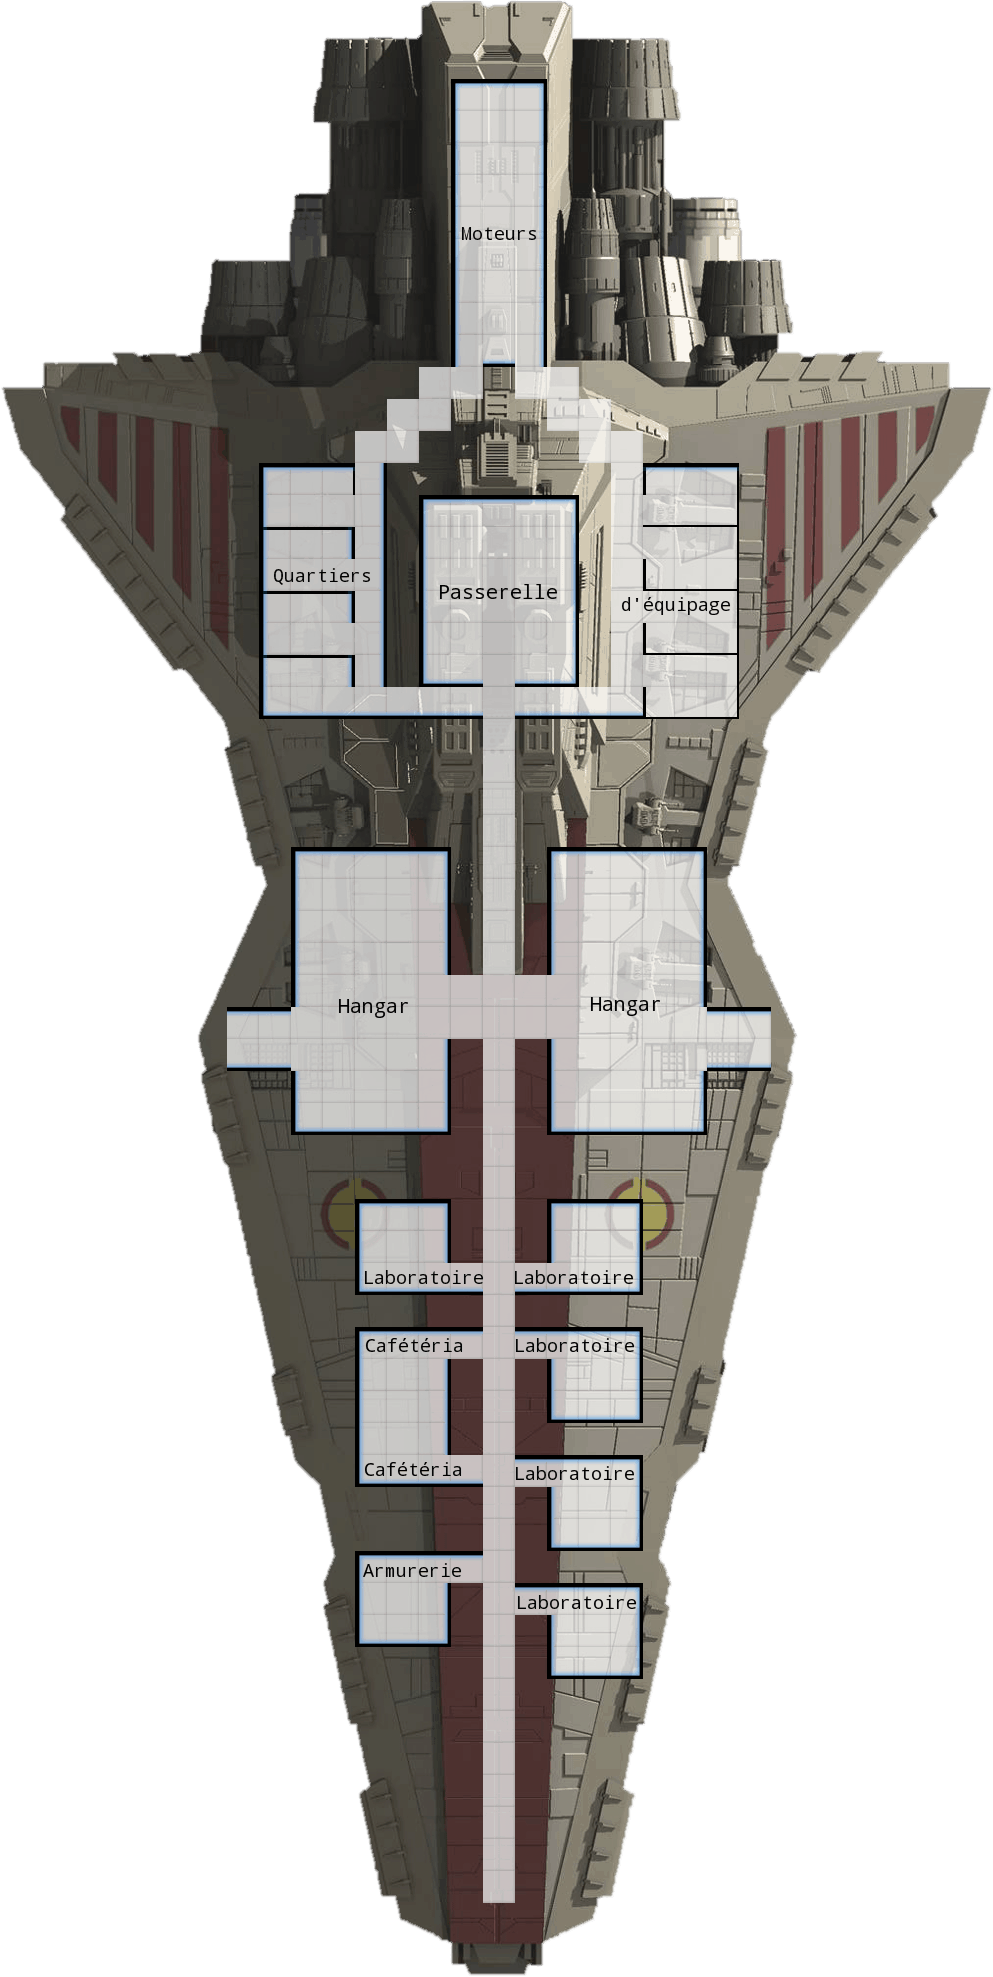
\includegraphics[width=\linewidth]{_img/dos-au-muur/venator-plan.png}

Ce n'est qu'une proposition, le plan peut changer à volonté. En annexe, vous trouverez des cases permettant de faire découvrire le vaisseau petit à petit aux héros.

\clearpage
\section{Bestiaire}

\subsection{Rakghoul}
\label{sec:rakghoul}
\noindent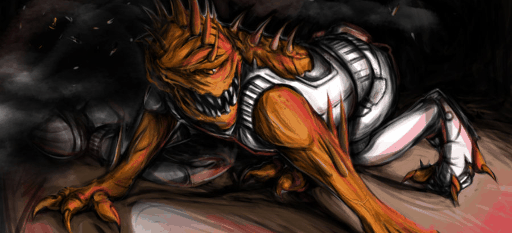
\includegraphics[width=\linewidth]{_img/dos-au-muur/rakghoul.png}

\subsubsection{Traits}

\begin{itemtable}[ c c c c c ]
    \textbf{Agi} & \textbf{Int} & \textbf{\^Ame} & \textbf{For} & \textbf{Vig} \\
    d8			 & d6			& d6			 & d8			& d8
\end{itemtable}
\begin{itemtable}[ l X ]
	\textbf{Allure} 	 & 6 \\
	~   				 & Vision Nocturne \\
	~   				 & Marche sur les murs \\
	\textbf{Compétences} & Combat d8, Discrétion d6
\end{itemtable}

\subsubsection{Défense}
\begin{itemtable}[ c c ]
	\textbf{Parade} 	& \textbf{Résistance} \\
	6					& 6 
\end{itemtable}

\subsubsection{Attaque}
\begin{itemtable}[ X c c ]
	~ 		& \textbf{Combat} 	& \textbf{Dégats} \\
	Griffes	& d8 				& 1d6 
\end{itemtable}

\newpage
\subsubsection{Background}
Les Rakghouls sont une espèce issue d'une maladie créée par le seigneur Sith Karness Muur. Les individus ateint par cette maladie deviennent des monstres incapable de penser par eux même. Karness peut les contrôller grâce à son talisman (Le Talisman de Muur).

La maladie se transmet par une griffure ou un morsure mais cela ne fonctionne pas avec les êtres sensibles à la Force. Karness a créé se virus à partir du coté Obscur de la Force ce qui explique une forte présence obscure près de ces monstres.

Karness a créé plusieurs versions du virus car les premiers Rakghouls ne répondaient pas bien au contrôle de Karness. Les nouveaux sont plus réceptif et plus fort.

Quand le Talisman de Muur a été perdu dans les bas fonds de Taris, on a peu constaté que les créatures, suite à une exposition prologé au Talisman finissaient par se transformer en Rakghouls. Mais les Rakghouls transformé de cette façon sont bestiaux, stupide et sans âme. Ils attaquent tout ce qui bouge. Ces créatures ne fonctionne qu'à l'instinct.

\clearpage
\subsection{Rakghoul Amblyope}
\label{sec:rakghoul-amblyope}
\noindent
\includegraphics[width=\linewidth]{_img/dos-au-muur/rakghoul-amblyope.png}

\subsubsection{Traits}

\begin{itemtable}[ c c c c c ]
    \textbf{Agi} & \textbf{Int} & \textbf{\^Ame} & \textbf{For} & \textbf{Vig} \\
    d4			 & d6			& d6			 & d12+2		& d10
\end{itemtable}
\begin{itemtable}[ l X ]
	\textbf{Allure} 	 & 5 \\
	\textbf{Taille} 	 & +5 \\
	~   				 & Vision de Force \\
	~					 & \'Enorme (+2 pour les jets d'attaque adverses)\\
	\textbf{Compétences} & Combat d10
\end{itemtable}

\subsubsection{Défense}
\begin{itemtable}[ c c ]
	\textbf{Parade} 	& \textbf{Résistance} \\
	5					& 12 
\end{itemtable}

\subsubsection{Attaque}
\begin{itemtable}[ X c c ]
	~ 			& \textbf{Combat} 	& \textbf{Dégats} \\
	Mains nues	& d10 				& d12+2 
\end{itemtable}

\newpage
\subsubsection{Background}
Version stéroïdé des Rakghouls standard, Amblyope est notre petit boss de niveau.

Quand les Rakghouls sont livrés à eux mêmes et qu'il laisse libre court à leurs plus bas instincts, il arrive qu'un Rakghoul plus fort que les autres s'en prenne à ces petits camarades et les dévore sans scrupule. Cette afflut de Force Obscure peut le faire muter et le Rakghoul devient une espèce de gros monstre de 3m de haut, complètement aveugle mais attiré par les émanation de Force, il attaque machinalement les adversaires les plus sensible à la Force. 

\clearpage
\subsection{Vyna Anen}
\noindent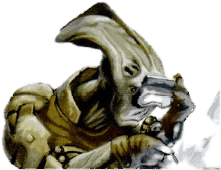
\includegraphics[width=\linewidth]{_img/dos-au-muur/vyna-anen.png}

\subsubsection{Traits}

\begin{itemtable}[ c c c c c ]
    \textbf{Agi} & \textbf{Int} & \textbf{\^Ame} & \textbf{For} & \textbf{Vig} \\
    d6			 & d10			& d6			 & d4			& d6
\end{itemtable}
\begin{itemtable}[ l X ]
	\textbf{Allure} 	 & 6 \\
	\textbf{Compétences} & Intimidation d6, Persuasion d12, Réseaux d6
\end{itemtable}

\subsubsection{Défense}
\begin{itemtable}[ c c ]
	\textbf{Parade} 	& \textbf{Résistance} \\
	2					& 5 
\end{itemtable}

\newpage
\subsubsection{Background}
Vyna Anen est l'un des agent de liaison entre Industrial Automaton et l'Empire. Officiellement employé par IA comme secrétaire au service des "Projets Spéciaux". 

Vyna est un homme pragmatique qui fait ce que l'Empire lui demande sans poser de question, sans scrupule ni état d'âme. C'est une fin négociateur entièrement voué à l'Empire.\\

\noindent
\includegraphics[width=\linewidth]{_img/dos-au-muur/industrial-automaton.png}

\subsection{Droïde R4 [Joker]}



	\onecolumn
	\nocite{*}
	\printbibliography
\end{document}